\section{Herramientas}
\label{sec:herramientas}

Se recogen en esta sección, por otro lado, las principales herramientas empleadas durante el proceso \textit{software} ejecutado para la realización del presente TFG. El uso de estas herramientas tiene, en todos los casos, la finalidad de mejorar el rendimiento del proceso favoreciendo una mejor organización o introduciendo facilidades para el desarrollo \textit{software}.

\subsection{Herramientas para el producto}
\subsubsection{Edición de código}
\label{subsec:edicionCodigo}
Habitualmente, la edición del código se realiza en entornos de desarrollo integrados (IDE), que son aplicaciones que incluyen una ingente cantidad de utilidades y servicios que permiten a los desarrolladores la redacción del código de una forma más sencilla, facilitando así el proceso de desarrollo.

Por la naturaleza de los tres componentes que forman \textit{VSCode4Teaching} en la actualidad ---detallada en la \referenciaSeccion{sec:diseñoArquitectura}---, se han utilizado tres entornos diferentes.

\textbf{Visual Studio Code} \cite{Her_VSCode}, de Microsoft (distribuido bajo licencia MIT), ha sido el IDE más empleado durante el proceso de desarrollo, ya que uno de los componentes de la aplicación es una extensión para este IDE.

Por otro lado, \textbf{IntelliJ IDEA} \cite{Her_IntelliJ}, de JetBrains (gratuito para fines eduativos), ha sido el IDE empleado para el desarrollo del servidor, ya que es un entorno enfocado a la creación y confección de proyectos Java y, específicamente, de aplicaciones web basadas en Spring.

A estas herramientas se suma \textbf{WebStorm} \cite{Her_WebStorm}, un entorno de JetBrains hermano de IntelliJ IDEA destinado específicamente a la plataforma JavaScript y con soporte, además, para el lenguaje TypeScript. También es gratuito para fines eduativos, y ha sido el IDE empleado para el desarrollo de la aplicación web SPA.

\subsubsection{Visualización de base de datos}
De entre la ingente cantidad de herramientas que existen para la gestión gráfica de bases de datos MySQL, la empleada durante este TFG ha sido \textbf{DBeaver} \cite{Her_DBeaver}. Es una aplicación gratuita multiplataforma ---distribuida con licencia Apache 2.0--- orientada a desarrolladores y administradores de bases de datos y que soporta todos los SGBD relacionales más populares, entre los que se encuentra el empleado en este proyecto.

\subsubsection{Sistema de control de versiones}
\label{subsec:vcs}
Los sistemas de control de versiones permiten a los equipos de desarrollo obtener un seguimiento de las distintos cambios ejecutados sobre un proyecto, añadiendo diversas opciones para la gestión de solapamientos o conflictos y para la diversificación del desarrollo en distintas tareas realizables simultáneamente mediante el concepto de ``rama'' de desarrollo.

Uno de los más extendidos en la actualidad es \textbf{git}, que es un ``sistema de control de versiones distribuido, gratuito y de código abierto diseñado para manejar con velocidad y eficiencia desde proyectos pequeños hasta muy grandes'' \cite{Her_Git} que, además, se distribuye bajo licencia GNU 2.0 (siendo, por tanto, \textit{software} libre).

En particular, para la ejecución de este proyecto se ha utilizado un repositorio público alojado en \textbf{GitHub}, que es un servicio que añade a git capacidades adicionales mediante una interfaz gráfica intuitiva y fácil de utilizar. Es empleada por más de 83 millones de desarrolladores y en ella hay registrados más de 200 millones de repositorios, haciendo de ella ``la plataforma de desarrollo más grande del mundo en la actualidad'' \cite{Her_GitHub}.

La \referenciaSeccion{sec:distribDespliegue} introduce más detalles acerca de la distribución del código del proyecto \textit{VSCode4Teaching}.

\subsubsection{CI/CD}
\label{subsec:cicd}
CI/CD es la abreviatura de \textit{Continuous Integration/Continuous Deployment}, traducido del inglés como ``integración continua/despliegue continuo'' (o, en ocasiones, ``integración continua/entrega continua''). Es uno de los procesos incluidos en la filosofía \textit{DevOps}, que está conformada por ``un conjunto de prácticas, herramientas [...] que sirve para automatizar e integrar los procesos [...] del equipo de desarrollo y de tecnologías de la información'' \cite{Her_DevOps}.

Así, CI/CD permite ``automatizar el flujo de desarrollo del \textit{software} para desplegar código de mejor calidad con mayor frecuencia usando un proceso iterativo y continuo para compilar, probar y desplegar, previniendo la posterior aparición de errores y fallos en el código'' \cite{Her_CICD}.

En el caso de este proyecto se hace uso de la herramienta \textbf{Travis CI}, que es una plataforma que permite ``compilar, probar y desplegar el código fácil y rápidamente'' \cite{Her_Travis} y que es gratuita para proyectos de \textit{software} libre, tal como lo es \textit{VSCode4Teaching}.
Para ello, se introduce un fichero llamado \texttt{.travis-ci.yml} en la raíz del proyecto. Este contiene la información que permite compilar y desplegar la imagen Docker, divulgándola a través de Internet. En el \referenciaCodigo{cod:travis} se introduce una parte del mencionado fichero como muestra de ejemplo de la configuración para el uso de Travis CI.

\begin{lstlisting}[language=YAML,caption={Fragmento del fichero de configuración de Travis CI para desplegar y divulgar la versión 2.2.0 de \textit{VSCode4Teaching}.},label=cod:travis]
jobs:
    include:
        - name: V4T Server (Spring Boot)
            jdk: oraclejdk11
            [...]
            script:
                - "./mvnw clean package -B -q"
            after_script:
                - docker build -t vscode4teaching/vscode4teaching:2.2.0 .
                - docker build -t vscode4teaching/vscode4teaching:latest .
                - docker push vscode4teaching/vscode4teaching:2.2.0
                - docker push vscode4teaching/vscode4teaching:latest
        - name: V4T Extension (Node.js)
            node_js: 10.15.3
            [...]
            before_script:
                - cd ./vscode4teaching-extension
                - npm install --save-dev
            script:
                - npm test
[...]
\end{lstlisting}

\subsection{Organización del proceso: Trello}
\label{subsec:herTrello}
Se ha realizado el presente Trabajo Fin de Grado siguiendo un proceso \textit{software} de pequeñas iteraciones que queda detallado en la \referenciaSeccion{sec:metodologia}. Tal como se recoge en la citada sección, uno de los principios básicos seguidos para la organización del trabajo ha sido la utilización de un tablero de tipo Kanban para la visualización, división, distribución y jerarquía de las tareas.

Durante el transcurso del proceso, \textbf{Trello} ha sido la herramienta informática empleada para ejecutar esta organización. Trello es una plataforma de uso gratuito de Atlassian que permite ``gestionar proyectos y lograr cotas más altas de productividad independientemente de la dinámica de trabajo'' \cite{Her_Trello}.

\begin{figure}[h]
    \centering
    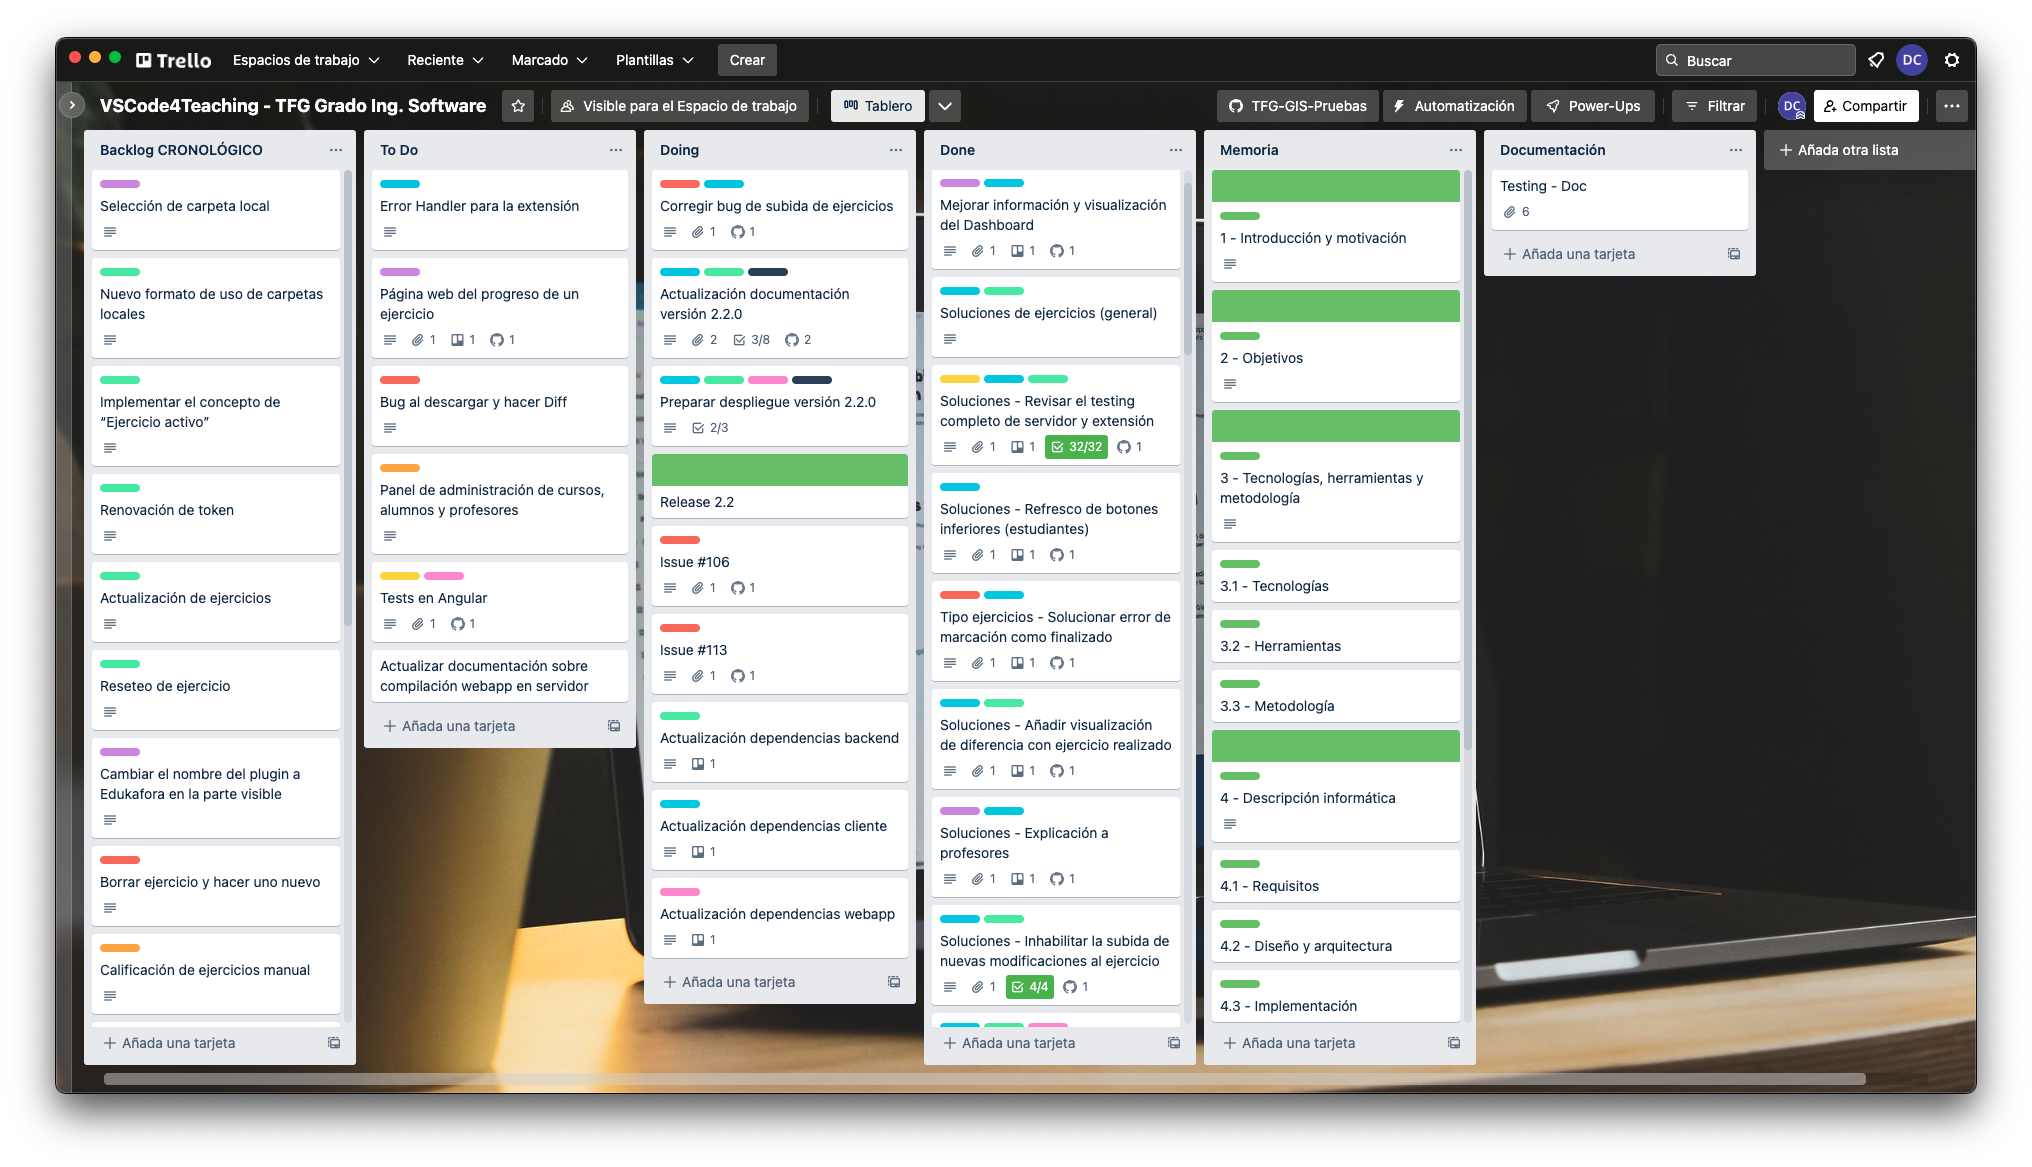
\includegraphics[width=\textwidth]{imagenes/utilizadas/3-2-herramientas/capturaTrello.png}
    \caption{Captura del tablero de trabajo Trello empleado.}
    \label{fig:Trello}
\end{figure}

La \referenciaFigura{fig:Trello} permite visualizar una captura del tablero empleado en Trello.
Esta herramienta permite la creación de diversas tarjetas representativas de tareas distribuidas en varias columnas a las que se les puede asignar fechas de inicio y finalización, así como etiquetas de distintos colores para su distinción temática, pudiendo además añadir comentarios y recursos adicionales ---hipervínculos, documentos adjuntos o enlaces hacia otras tarjetas asociadas, por ejemplo---. Mediante todas estas funcionalidades, esta herramienta permite a sus usuarios organizar de forma sencilla, intuitiva y muy visual el trabajo pendiente y realizado, facilitando la toma de decisiones de diseño y desarrollo y aumentando la productividad del tiempo dedicado.

Esta explicación queda ampliada en la \referenciaSeccion{sec:metodologia}, que aborda la forma de utilización del tablero Trello y su integración en el proceso de desarrollo seguido.
